\documentclass[main.tex]{subfiles}
\begin{document}
    \section{Hand curation of the floorplans}
    \subsection{Motivation}
		Upon observing  the variety of options for the initial floor-plan that could be used by the project, several issues were raised. The images available were often too complex for any immediate processing to take place and contained a lot of noise in the form of unknowns such as labels or icons. These kind of images were obviously not suitable for extraction of the floor plan and therefore it has been decided that in order to make use of the available resources, hand curation was necessary.
		\subsection{Selection of initial images}
		While there are many options when  obtaining the initial floor plans, such as requesting them from the university, we found out that floor-plans best suited for our needs could be obtained from the interactive map. These floor plans were a good fit for several reasons:
		
		\begin{itemize}
			\item They are a to-scale model, allowing us to rely on the proportions of the floor plan. This  was crucial for our needs as we needed to represent movement in real life on the image and if the proportions were different we would not be able to do so.
			\item The images contained additional information that benefited our application as well. This is the case with room numbers, symbols for utility rooms and others.
			\item Floor-plans for different buildings could be obtained with ease, allowing us to possibly expand the application to other buildings if need-be. This was a consideration for further testing should be run into issues with testing in DCS.
			\item They provided us with a good resource that could be utilized at later stages of our project, where we design our own floor plans in order to display information for the user.
		\end{itemize}
		
		\subsection{Process}
		The process of hand-curating the images involved the following steps:
		
		\begin{itemize}
			\item Limit a single room to one colour - This was a requirement as some rooms made use of gradient colours. Keeping these could greatly hinder the extraction process and the gradients were therefore removed
			\item Removal of labels and other text - The room numbers and other information will be stored in the graph itself and therefore were unnecessary when working on the extraction.
			\item Normalizing the colours of walls - Some of the walls and space outside the building were not completely white as they were dissolved by the gradients.
			\item Widen the doors in order to compensate for build-up error of sensors - This was necessary at the later stages of the project, where we realized that the build-up error of the sensors could stop us from navigating through doors.
		\end{itemize}
		
		\subsection{Benefits}
		Having a hand curated image allowed us to perform easier extraction of the navigation graph as well as introduced other possibilities on handling the further challenges in the implementation. The hand curated image is further used in wall-detection as well as other support systems for navigation. 
		
		\section{Graph extraction}
		\subsection{Considerations}
		When extracting the graph from the hand-curated images, the project encountered many issues related to the difference in performance of mobile devices as well as restrictions when processing specific device OS. It has been therefore decided to pre-extract all graphs from the images and only use the  post processed files in order to remove the on-device processing dependency. While this has downsides as well the performance cost is significantly smaller.
		\newline
		
	Another significant point when considering extracting the graph was the storage method on the device. Unlike PCs, phones and similar mobile devices utilize significantly smaller overall storage space and therefore we could not accommodate for large, dense and fine graphs. We were therefore forced to develop a method that would allow us to solve this problem. 
	\newline
	
The last significant part of our considerations for this process was representation of additional data present in the picture. We required a way how to navigate a user from specific rooms as well as allow for filtering of rooms per flood and similar. At the same time we had to balance the benefit gained from keeping data readily available in memory, and the limits on memory used by an application imposed by Android and iOS.
	\subsection{Initial approach}
	As per the decision explained in the previous section, all of the graph extraction was performed using a computer instead of real-time extraction on the device. This has allowed us to make use of heavy parallelism as well as methods exploiting non-PCL  libraries.
	\newline
	
Our initial version of the extraction algorithm utilized the hand curated graph we created by using a version of flood algorithm. This way performed by setting an initial point in the middle of the picture (or in any room)  and creating nodes and edges by flooding in 4 directions. This was bounded by simple logic, where no nodes were created in walls (white colour). While this approach provably worked, it had many performance issues due to objects in the .NET API - namely Bitmap. The GetPixel method was not thread safe and therefore was locking the Bitmap data before accessing it. It was therefore obvious that the subsequent iterations that will require more than a single iteration over all of the elements will have to overcome this problem
	\subsection{Optimisation}
	While the initial tool was capable of extracting a graph from the image, it caused many issues in regards to runtime and the overall size of the graph produced. In order to mend these problems we have decided to re-implement the tool with the issues from the previous version in mind. 
	\subsubsection{Removing the bitmap object dependency}
	The only way how to expose pixel data in the Bitmap object was to use its GetPixel method. This method is not thread safe and is therefore locking. This is caused issues when an attempt at using parallelism with the project was made. In order to remedy this, raw data of the bitmap image was stored in a two dimensional array, expressing information about the image. Thanks to this we were not only able to access the pixel information from multiple threads at once, but also ensure that the access time for an individual pixel is O(1) thanks to direct indexing. 
	\subsubsection{Node distance}
	In the vanilla version, each pixel represented a node in the graph. After running tests and comparing the measures , it became apparent that this approach is not feasible due to three separate reasons:
	
	\begin{itemize}
		\item Produced graph was too large - the graph created using this method contained up to 2,5 milion nodes. This has resulted in overall graph sizes over 150 MB, which is an unreasonable demand for a mobile device.
		\item Loading the graph on the device took too long due to the need to deserialize nodes and edges.
		\item The graph-pathfinding library used was struggling with the large amount of nodes and vertices, delaying the response time from a few hundred milliseconds to a few seconds. This was not suitable for real-time navigation.
	\end{itemize}
	

	\subsubsection{Two-directional linking}
	
	The initial version was forcing each node to check all four directions for possible neighbours. This was redundant as the same effect could be achieved by ckecking only two directions in an undirected graph. The solution was therefore adapted to only check left and right from each node created in search for neighbours.
	\subsubsection{Introduction of multi-pass graph generation}
	The initial version also suffered from severe inter-loop dependency. This was caused by the fact that in order to create an edge, all of the vertices had to be already created - otherwise we could miss some of them. This caused the separate threads to block each other. In order to resolve this, multi-pass was adapted.  The optimised version therefore processes separate stages sequentially, while each individual stage exploits paralelism.
	\subsection{Runtime summary}
	The optimisations greatly improved the runtime of the extraction. Thanks to the usage of direct indexing and hashing, we were able to ensure that the extraction process didn't take longer than a few seconds to perform all the steps necessary in order to generate a graph that can be navigated across. The initial generation of nodes for the graph runs in the time O(n) as it needs to check each position on the image for a possible node. Each operation with pixels runs in O(1) thanks to the ability to directly index into the pre-processed array. The linking operation runs in a combined time of O(n * log(n)) + O(2n) due to the need to check two directions for possible links as well as locating a node in a collection. The collection of nodes is represented by a Dictionary type, which loosely translates to a HashMap. 
	\subsection{Saving and loading}
	The project utilizes XML as its means of storage. This is due to multiple reasons:
	
	\begin{itemize}
		\item The robust nature of XML based storage is a good match for this project as its ensures validity checking as well as allows for easier understanding of the data present. Using this approach also opened up the graph datastructure to modifications beyond the scope of edge and vertex data. 
		\item The language we chose - C\# - has great support for XML data. It allowed us to utilize serialisation and deserialisation of objects into XML, resulting in easier integration and faster loading times.
	\end{itemize}
	\subsection{Benefits \& Limitations}
	By implementing our own custom extraction as well as loading and saving methods for the graph, we have managed to work around the restrictions imposed by the existing methods and utilize the full potential of having access to floor plan data. Our decision to keep room data and navigation data in separate files further allowed us to allow the application to handle arbitrary amount of floors, by simply having a reference handle to files that involve navigation without loading the floor plan into memory. The finalized data storage method is flexible and therefore can be updated at later stages without the need to re-generate all floors for a given building.
\newline

The extraction method was heavily optimised for speed using only a few steps to reach the final graph as shown in \textbf{Figure[\ref{fig:nav_graph}]}. This approach was adapted to ensure we can extract floor plans from different buildings for later tests, if need be. This has encouraged us to make heavy use of parallelism in our extraction process as well as a series of methods that allow us to access image data directly. 
\newline

By utilizing the methods explained above, we were aiming to decrease the amount of processing required to be performed on the device and this should therefore benefit user experience. We encountered several issues with mobile devices, where in both cases iOS and Android we reached the maximum memory allowed per-application and therefore had to re-design our approach to loading floor plans multiple repeatedly, eventually arriving at an optimal solution.
\begin{figure}[h]
\center
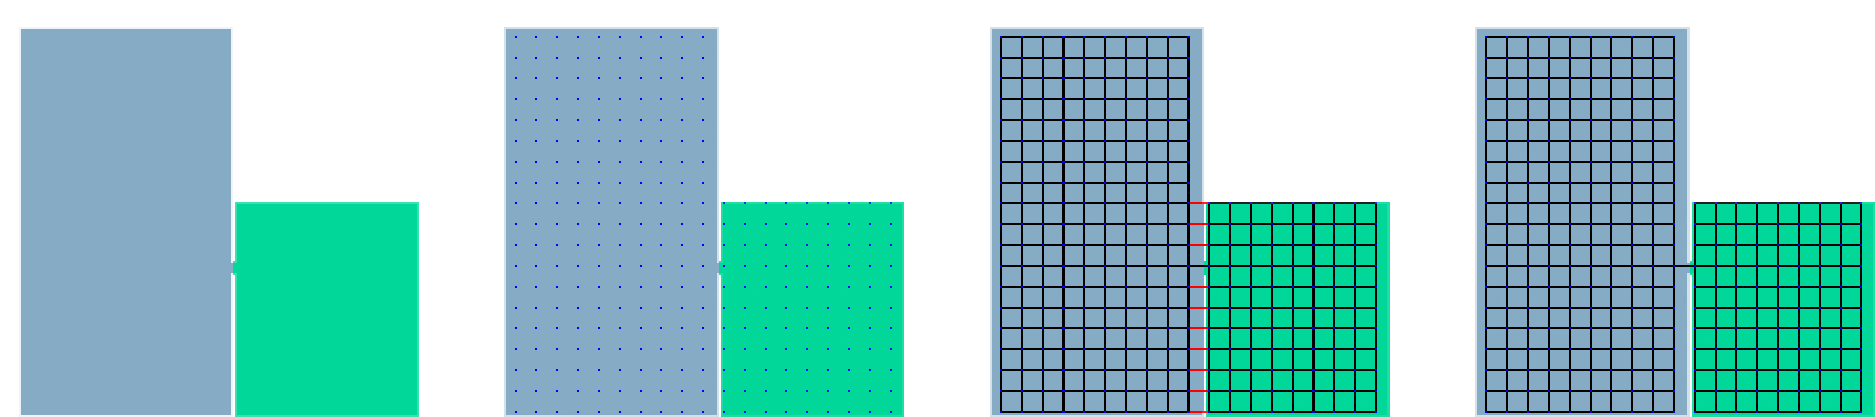
\includegraphics[trim=0 0 0 0, clip,width=\textwidth,height=\textheight,keepaspectratio]{images/graphGeneration.pdf}
\caption{Steps in generation of the pathfinding graph, from the initial hand curated image to full navigational graph.}
\label{fig:nav_graph}
\end{figure}
\end{document}
